In offline performance, there was very little difference between the best-performing proposed function and \tloA{}. For this reason, the remainder of the results reported will discuss performance during online testing, i.e., performance during learning itself.% and Offline testing\footnote{did we meantion what those words mean, did we even mention learning before?}. 


\begin{table}[t]
\footnotesize
  \caption{Mean $\text{R}^*$ Online performance. Each row represents comparable performance across 5 different objective functions. Values within 10\% of the best value in each row are highlighted. Higher scores are better. Items are significantly different from \tloA{} when marked *$p<0.05$, ** $p <0.01$, *** $p<0.001$; arrows mark the direction of significant differences.}
  \label{tab:mean_r_star_performance}
  %\resizebox{5cm}{!}{
\begin{tabular}{>{\raggedright\arraybackslash}p{5em}>{\raggedleft\arraybackslash}p{4em}>{\raggedright\arraybackslash}p{4.5em}rrrrr}
\toprule
Environment & Objective Modified & Objective Scale & EEBA1 & ROLF_EXP_LOG1 & SEBA & SFELLA & TLO$^A$\\
\midrule
 &  & 1 & 1.40** & 4.08*** & \textcolor{black}{1.43**} & \textcolor{blue}{6.54***} & \textcolor{black}{1.81}\\
\cmidrule{2-8}
 &  & 0.01 & 1.27 & 4.39*** & \textcolor{black}{1.33} & \textcolor{black}{1.38} & \textcolor{black}{1.46}\\

 &  & 0.1 & 1.38 & 4.21*** & \textcolor{black}{1.39} & \textcolor{black}{1.88**} & \textcolor{black}{1.41}\\

 &  & 10 & 6.08*** & 3.45*** & \textcolor{blue}{6.32***} & \textcolor{black}{4.44***} & \textcolor{black}{-0.22}\\

 & \multirow[t]{-4}{4em}{\raggedleft\arraybackslash Alignment} & 100 & -7.12*** & -4.08*** & \textcolor{blue}{2.22***} & \textcolor{black}{-3.49***} & \textcolor{black}{-0.48}\\
\cmidrule{2-8}
 &  & 0.01 & 5.85*** & 5.45*** & \textcolor{blue}{6.34***} & \textcolor{black}{5.51***} & \textcolor{black}{1.96}\\

 &  & 0.1 & 5.89*** & 5.38*** & \textcolor{black}{2.46**} & \textcolor{blue}{6.43***} & \textcolor{black}{1.88}\\

 &  & 10 & 1.50* & -14.73*** & \textcolor{black}{1.41**} & \textcolor{blue}{6.51***} & \textcolor{black}{1.77}\\

\multirow[t]{-9}{5em}{\raggedright\arraybackslash Breakable Bottles} & \multirow[t]{-4}{4em}{\raggedleft\arraybackslash Performance} & 100 & 1.48* & -12.83*** & \textcolor{black}{1.46**} & \textcolor{blue}{6.40***} & \textcolor{black}{1.81}\\
\cmidrule{1-8}
 &  & 1 & 1.47*** & -9.33*** & \textcolor{black}{-0.48***} & \textcolor{blue}{4.38***} & \textcolor{black}{3.87}\\
\cmidrule{2-8}
 &  & 0.01 & -0.76** & -9.34*** & \textcolor{black}{-0.73*} & \textcolor{black}{-0.58} & \textcolor{black}{-0.49}\\

 &  & 0.1 & -0.54 & -9.32*** & \textcolor{black}{-0.64} & \textcolor{blue}{8.29***} & \textcolor{black}{-0.63}\\

 &  & 10 & 3.53 & -9.71*** & \textcolor{blue}{3.43} & \textcolor{blue}{3.74} & \textcolor{blue}{3.63}\\

 & \multirow[t]{-4}{4em}{\raggedleft\arraybackslash Alignment} & 100 & 3.59*** & -9.88*** & \textcolor{black}{3.16**} & \textcolor{black}{2.73} & \textcolor{black}{2.82}\\
\cmidrule{2-8}
 &  & 0.01 & 3.70** & 3.59*** & \textcolor{black}{3.43***} & \textcolor{black}{3.66***} & \textcolor{blue}{4.09}\\

 &  & 0.1 & 4.36*** & 3.67* & \textcolor{blue}{5.39***} & \textcolor{black}{4.10} & \textcolor{black}{3.91}\\

 &  & 10 & -0.40*** & -14.18*** & \textcolor{black}{-0.70***} & \textcolor{blue}{4.41***} & \textcolor{blue}{3.97}\\

\multirow[t]{-9}{5em}{\raggedright\arraybackslash Doors} & \multirow[t]{-4}{4em}{\raggedleft\arraybackslash Performance} & 100 & -0.71*** & -13.75*** & \textcolor{black}{-0.51***} & \textcolor{blue}{4.17**} & \textcolor{blue}{3.85}\\
\cmidrule{1-8}
 &  & 1 & -15.03*** & 5.28*** & \textcolor{black}{-14.98***} & \textcolor{black}{-10.29***} & \textcolor{blue}{10.76}\\
\cmidrule{2-8}
 &  & 0.01 & -14.99 & 2.81*** & \textcolor{black}{-15.02} & \textcolor{black}{-14.97} & \textcolor{black}{-14.97}\\

 &  & 0.1 & -15.00 & 4.80*** & \textcolor{black}{-14.96} & \textcolor{black}{-14.98} & \textcolor{black}{-14.95}\\

 &  & 10 & 10.89*** & 3.43*** & \textcolor{blue}{10.88***} & \textcolor{blue}{10.92***} & \textcolor{blue}{10.72}\\

 & \multirow[t]{-4}{4em}{\raggedleft\arraybackslash Alignment} & 100 & 3.55*** & -0.10*** & \textcolor{blue}{10.82***} & \textcolor{black}{3.76***} & \textcolor{blue}{10.49}\\
\cmidrule{2-8}
 &  & 0.01 & 10.83 & 10.86* & \textcolor{blue}{10.91***} & \textcolor{blue}{10.86*} & \textcolor{blue}{10.77}\\

 &  & 0.1 & -14.99*** & 10.82 & \textcolor{black}{-14.96***} & \textcolor{black}{5.97***} & \textcolor{blue}{10.82}\\

 &  & 10 & -15.00*** & -5.30*** & \textcolor{black}{-15.01***} & \textcolor{black}{-11.05***} & \textcolor{blue}{10.88}\\

\multirow[t]{-9}{5em}{\raggedright\arraybackslash Sokoban} & \multirow[t]{-4}{4em}{\raggedleft\arraybackslash Performance} & 100 & -14.96*** & -6.69*** & \textcolor{black}{-14.96***} & \textcolor{black}{-10.97***} & \textcolor{blue}{10.82}\\
\cmidrule{1-8}
 &  & 1 & 28.70*** & 16.35*** & \textcolor{blue}{28.71***} & \textcolor{blue}{27.99***} & \textcolor{blue}{27.09}\\
\cmidrule{2-8}
 &  & 0.01 & 28.76 & 16.82*** & \textcolor{blue}{28.70} & \textcolor{blue}{28.73} & \textcolor{blue}{28.79}\\

 &  & 0.1 & 28.75 & 16.51*** & \textcolor{blue}{28.72} & \textcolor{blue}{28.74} & \textcolor{blue}{28.72}\\

 &  & 10 & 27.15*** & 15.81*** & \textcolor{blue}{27.62***} & \textcolor{blue}{25.90***} & \textcolor{black}{23.37}\\

 & \multirow[t]{-4}{4em}{\raggedleft\arraybackslash Alignment} & 100 & 25.27*** & 14.91 & \textcolor{blue}{25.66***} & \textcolor{black}{18.67***} & \textcolor{black}{14.60}\\
\cmidrule{2-8}
 &  & 0.01 & 27.04 & 26.75** & \textcolor{blue}{27.73***} & \textcolor{blue}{26.79*} & \textcolor{blue}{26.98}\\

 &  & 0.1 & 28.61*** & 26.48*** & \textcolor{blue}{28.66***} & \textcolor{blue}{27.82***} & \textcolor{blue}{27.15}\\

 &  & 10 & 28.70*** & 7.50*** & \textcolor{blue}{28.78***} & \textcolor{blue}{27.91***} & \textcolor{blue}{27.10}\\

\multirow[t]{-9}{5em}{\raggedright\arraybackslash Unbreakable Bottles} & \multirow[t]{-4}{4em}{\raggedleft\arraybackslash Performance} & 100 & 28.69*** & 16.01*** & \textcolor{blue}{28.75***} & \textcolor{blue}{27.85***} & \textcolor{blue}{27.08}\\
\bottomrule
\end{tabular}
}
%\begin{adjustbox}{width=0.8\columnwidth,center}%
\begin{adjustbox}{width=\columnwidth}

\begin{tabular}{>{\raggedright\arraybackslash}p{5em}>{\raggedleft\arraybackslash}p{4em}>{\raggedright\arraybackslash}p{4.5em}rrrr}
\toprule
Environment & Objective Modified & Objective Scale & SEBA & SFELLA & LinearSum & TLO$^A$\\
\midrule
 &  & 1 & \textcolor{black}{1.43$\downarrow$**} & \textcolor{blue}{6.54$\uparrow$***} & \textcolor{black}{1.48$\downarrow$*} & \textcolor{black}{1.81}\\
\cmidrule{2-7}
 &  & 0.01 & \textcolor{black}{1.33} & \textcolor{black}{1.38} & \textcolor{black}{1.47} & \textcolor{black}{1.46}\\

 &  & 0.1 & \textcolor{black}{1.39} & \textcolor{black}{1.88$\uparrow$**} & \textcolor{black}{1.37} & \textcolor{black}{1.41}\\

 &  & 10 & \textcolor{blue}{6.32$\uparrow$***} & \textcolor{black}{4.44$\uparrow$***} & \textcolor{black}{5.61$\uparrow$***} & \textcolor{black}{-0.22}\\

 & \multirow[t]{-4}{4em}{\raggedleft\arraybackslash Alignment} & 100 & \textcolor{black}{2.22$\uparrow$***} & \textcolor{black}{-3.49$\downarrow$***} & \textcolor{blue}{6.05$\uparrow$***} & \textcolor{black}{-0.48}\\
\cmidrule{2-7}
 &  & 0.01 & \textcolor{blue}{6.34$\uparrow$***} & \textcolor{black}{5.51$\uparrow$***} & \textcolor{blue}{6.01$\uparrow$***} & \textcolor{black}{1.96}\\

 &  & 0.1 & \textcolor{black}{2.46$\uparrow$**} & \textcolor{blue}{6.43$\uparrow$***} & \textcolor{black}{5.43$\uparrow$***} & \textcolor{black}{1.88}\\

 &  & 10 & \textcolor{black}{1.41$\downarrow$**} & \textcolor{blue}{6.51$\uparrow$***} & \textcolor{black}{1.44$\downarrow$*} & \textcolor{black}{1.77}\\

\multirow[t]{-9}{5em}{\raggedright\arraybackslash BB} & \multirow[t]{-4}{4em}{\raggedleft\arraybackslash Primary} & 100 & \textcolor{black}{1.46$\downarrow$**} & \textcolor{blue}{6.40$\uparrow$***} & \textcolor{black}{1.35$\downarrow$***} & \textcolor{black}{1.81}\\
\cmidrule{1-7}
 &  & 1 & \textcolor{black}{-0.48$\downarrow$***} & \textcolor{black}{4.38$\uparrow$***} & \textcolor{black}{-0.47$\downarrow$***} & \textcolor{black}{3.87}\\
\cmidrule{2-7}
 &  & 0.01 & \textcolor{black}{-0.73$\downarrow$*} & \textcolor{black}{-0.58} & \textcolor{black}{-0.48} & \textcolor{black}{-0.49}\\

 &  & 0.1 & \textcolor{black}{-0.64} & \textcolor{blue}{8.29$\uparrow$***} & \textcolor{black}{-0.52} & \textcolor{black}{-0.63}\\

 &  & 10 & \textcolor{black}{3.43} & \textcolor{black}{3.74} & \textcolor{blue}{5.75$\uparrow$***} & \textcolor{black}{3.63}\\

 & \multirow[t]{-4}{4em}{\raggedleft\arraybackslash Alignment} & 100 & \textcolor{black}{3.16$\uparrow$**} & \textcolor{black}{2.73} & \textcolor{black}{3.95$\uparrow$***} & \textcolor{black}{2.82}\\
\cmidrule{2-7}
 &  & 0.01 & \textcolor{black}{3.43$\downarrow$***} & \textcolor{black}{3.66$\downarrow$***} & \textcolor{black}{4.05} & \textcolor{black}{4.09}\\

 &  & 0.1 & \textcolor{black}{5.39$\uparrow$***} & \textcolor{black}{4.10} & \textcolor{blue}{5.71$\uparrow$***} & \textcolor{black}{3.91}\\

 &  & 10 & \textcolor{black}{-0.70$\downarrow$***} & \textcolor{blue}{4.41$\uparrow$***} & \textcolor{black}{-0.67$\downarrow$***} & \textcolor{blue}{3.97}\\

\multirow[t]{-9}{5em}{\raggedright\arraybackslash Doors} & \multirow[t]{-4}{4em}{\raggedleft\arraybackslash Primary} & 100 & \textcolor{black}{-0.51$\downarrow$***} & \textcolor{blue}{4.17$\uparrow$**} & \textcolor{black}{-0.58$\downarrow$***} & \textcolor{blue}{3.85}\\
\cmidrule{1-7}
 &  & 1 & \textcolor{black}{-14.98$\downarrow$***} & \textcolor{black}{-10.29$\downarrow$***} & \textcolor{black}{-14.97$\downarrow$***} & \textcolor{blue}{10.76}\\
\cmidrule{2-7}
 &  & 0.01 & \textcolor{black}{-15.02} & \textcolor{black}{-14.97} & \textcolor{black}{-14.98} & \textcolor{black}{-14.97}\\

 &  & 0.1 & \textcolor{black}{-14.96} & \textcolor{black}{-14.98} & \textcolor{black}{-14.99} & \textcolor{black}{-14.95}\\

 &  & 10 & \textcolor{blue}{10.88$\uparrow$***} & \textcolor{blue}{10.92$\uparrow$***} & \textcolor{black}{-14.95$\downarrow$***} & \textcolor{blue}{10.72}\\

 & \multirow[t]{-4}{4em}{\raggedleft\arraybackslash Alignment} & 100 & \textcolor{blue}{10.82$\uparrow$***} & \textcolor{black}{3.76$\downarrow$***} & \textcolor{blue}{10.86$\uparrow$***} & \textcolor{blue}{10.49}\\
\cmidrule{2-7}
 &  & 0.01 & \textcolor{blue}{10.91$\uparrow$***} & \textcolor{blue}{10.86$\uparrow$*} & \textcolor{blue}{10.82} & \textcolor{blue}{10.77}\\

 &  & 0.1 & \textcolor{black}{-14.96$\downarrow$***} & \textcolor{black}{5.97$\downarrow$***} & \textcolor{black}{-14.95$\downarrow$***} & \textcolor{blue}{10.82}\\

 &  & 10 & \textcolor{black}{-15.01$\downarrow$***} & \textcolor{black}{-11.05$\downarrow$***} & \textcolor{black}{-14.98$\downarrow$***} & \textcolor{blue}{10.88}\\

\multirow[t]{-9}{5em}{\raggedright\arraybackslash Sokoban} & \multirow[t]{-4}{4em}{\raggedleft\arraybackslash Primary} & 100 & \textcolor{black}{-14.96$\downarrow$***} & \textcolor{black}{-10.97$\downarrow$***} & \textcolor{black}{-14.97$\downarrow$***} & \textcolor{blue}{10.82}\\
\cmidrule{1-7}
 &  & 1 & \textcolor{blue}{28.71$\uparrow$***} & \textcolor{blue}{27.99$\uparrow$***} & \textcolor{blue}{28.76$\uparrow$***} & \textcolor{blue}{27.09}\\
\cmidrule{2-7}
 &  & 0.01 & \textcolor{blue}{28.70} & \textcolor{blue}{28.73} & \textcolor{blue}{28.74} & \textcolor{blue}{28.79}\\

 &  & 0.1 & \textcolor{blue}{28.72} & \textcolor{blue}{28.74} & \textcolor{blue}{28.77} & \textcolor{blue}{28.72}\\

 &  & 10 & \textcolor{blue}{27.62$\uparrow$***} & \textcolor{blue}{25.90$\uparrow$***} & \textcolor{blue}{28.72$\uparrow$***} & \textcolor{black}{23.37}\\

 & \multirow[t]{-4}{4em}{\raggedleft\arraybackslash Alignment} & 100 & \textcolor{blue}{25.66$\uparrow$***} & \textcolor{black}{18.67$\uparrow$***} & \textcolor{blue}{27.42$\uparrow$***} & \textcolor{black}{14.60}\\
\cmidrule{2-7}
 &  & 0.01 & \textcolor{blue}{27.73$\uparrow$***} & \textcolor{blue}{26.79$\downarrow$*} & \textcolor{blue}{27.31$\uparrow$***} & \textcolor{blue}{26.98}\\

 &  & 0.1 & \textcolor{blue}{28.66$\uparrow$***} & \textcolor{blue}{27.82$\uparrow$***} & \textcolor{blue}{28.64$\uparrow$***} & \textcolor{blue}{27.15}\\

 &  & 10 & \textcolor{blue}{28.78$\uparrow$***} & \textcolor{blue}{27.91$\uparrow$***} & \textcolor{blue}{28.69$\uparrow$***} & \textcolor{blue}{27.10}\\

\multirow[t]{-9}{5em}{\raggedright\arraybackslash UB} & \multirow[t]{-4}{4em}{\raggedleft\arraybackslash Primary} & 100 & \textcolor{blue}{28.75$\uparrow$***} & \textcolor{blue}{27.85$\uparrow$***} & \textcolor{blue}{28.71$\uparrow$***} & \textcolor{blue}{27.08}\\
\bottomrule
\end{tabular}

\end{adjustbox}
\end{table}

% \begin{figure*}[h]
 
%   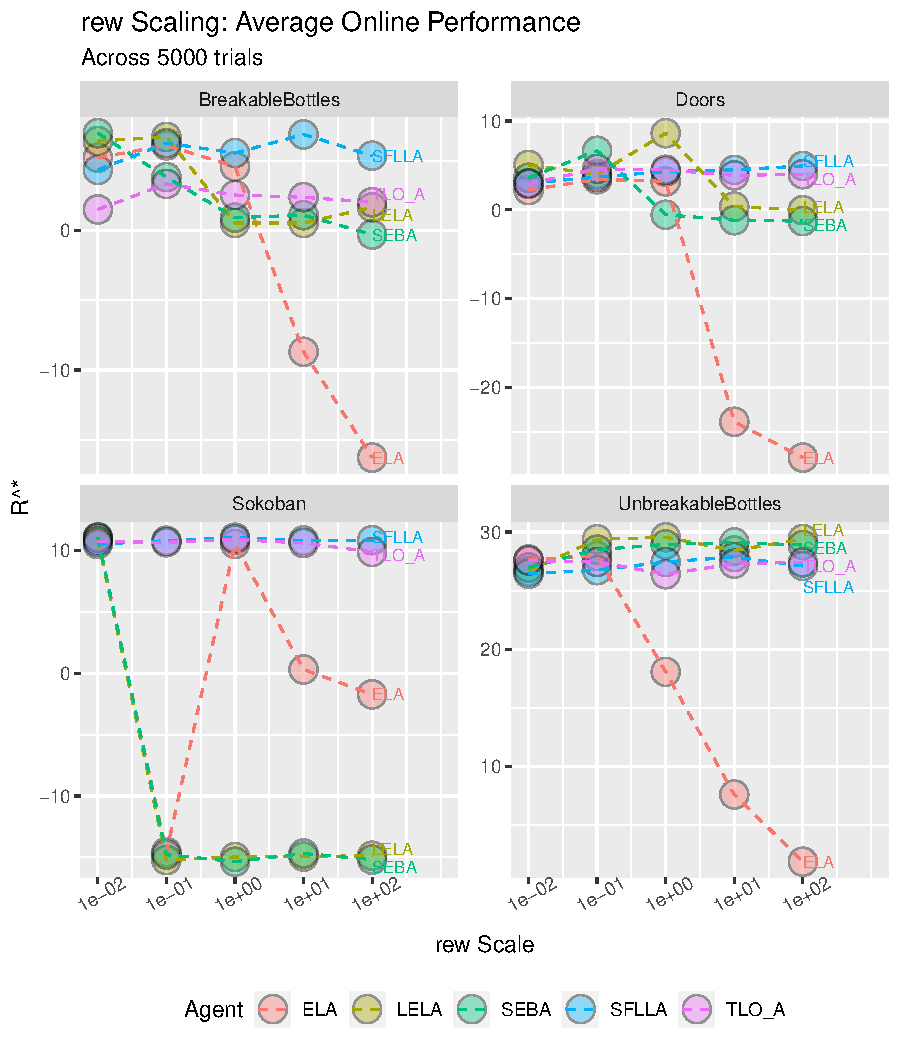
\includegraphics[width=\columnwidth]{output/onlinerew.pdf}
%   \caption{Online Reward scaled performance}
%   \label{fig:offline_pen_performance}
%   \Description{Online Reward scaled performance}
% \end{figure*}

% \begin{figure}[h]
%   %\centering
%   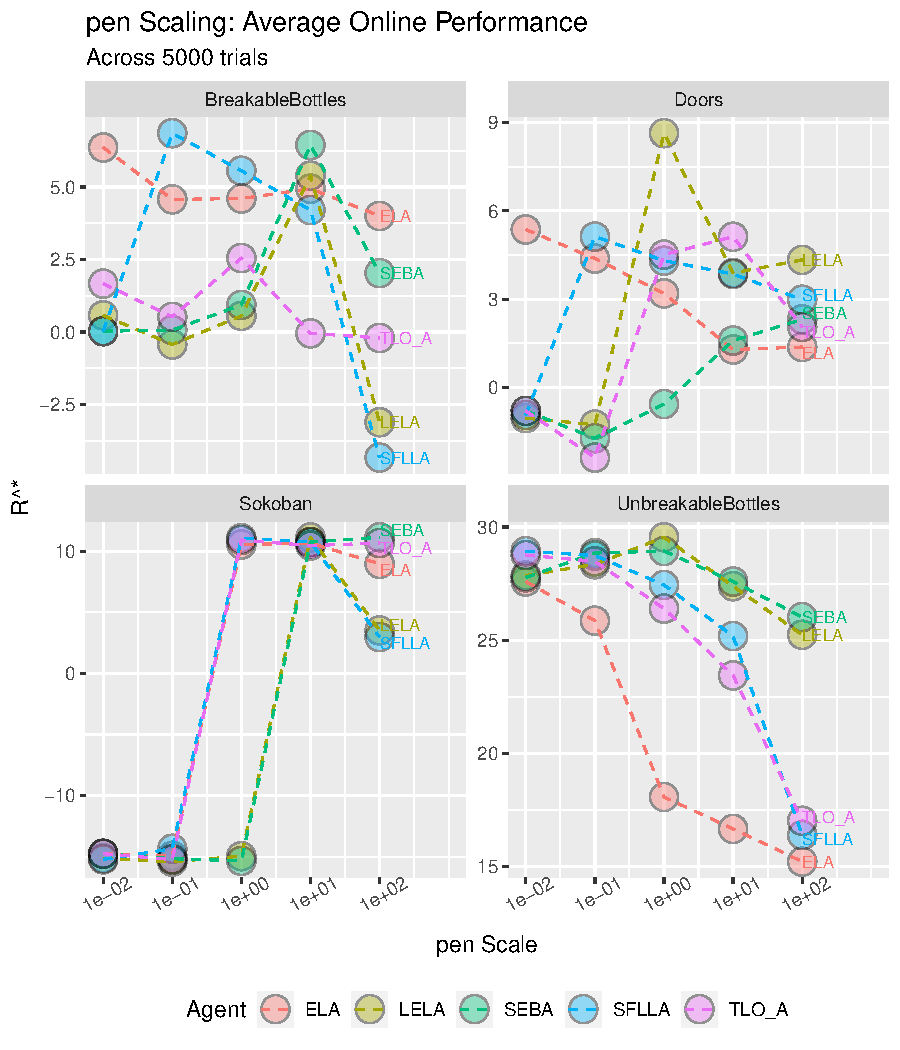
\includegraphics[width=\columnwidth]{output/onlinepen.pdf}
%   \caption{Online penalty scaled performance}
%   \label{fig:offline_pen_performance2}
%   \Description{Online penalty scaled performance}
% \end{figure}

\begin{figure}
  %\centering
  %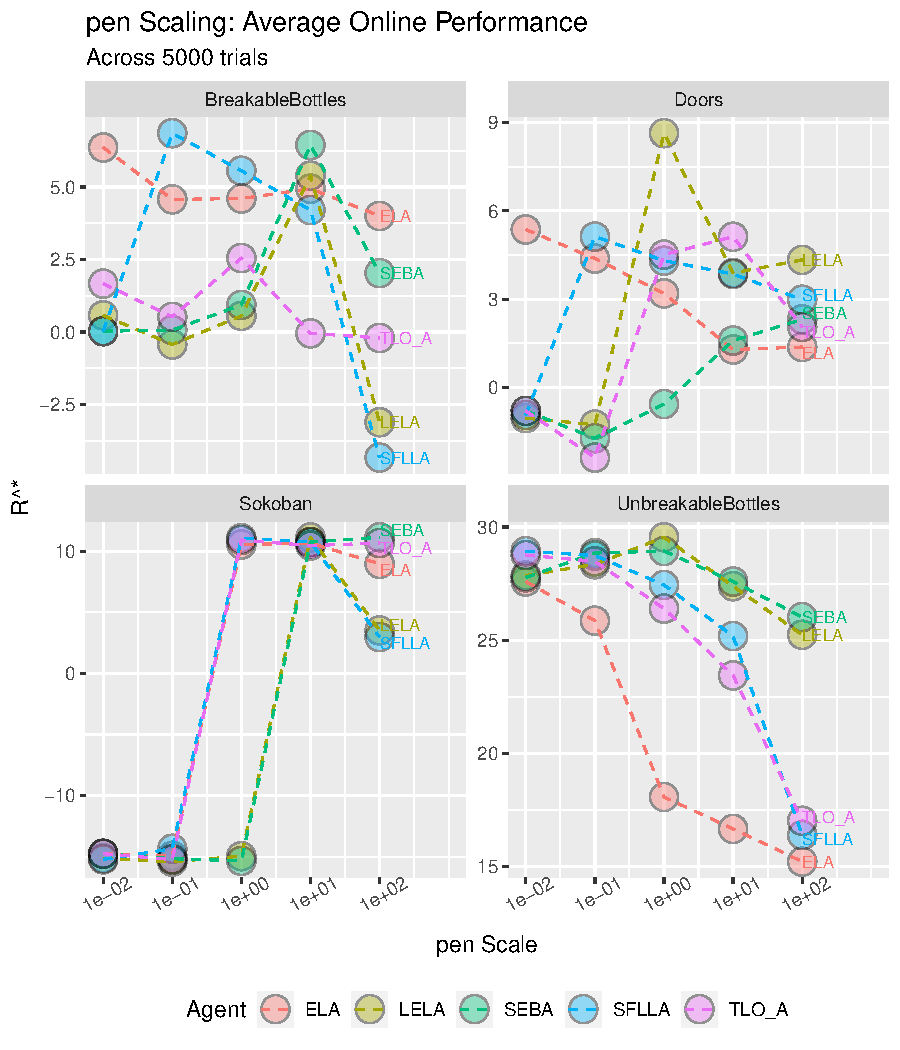
\includegraphics[width=\columnwidth]{output/onlinepen.pdf}
  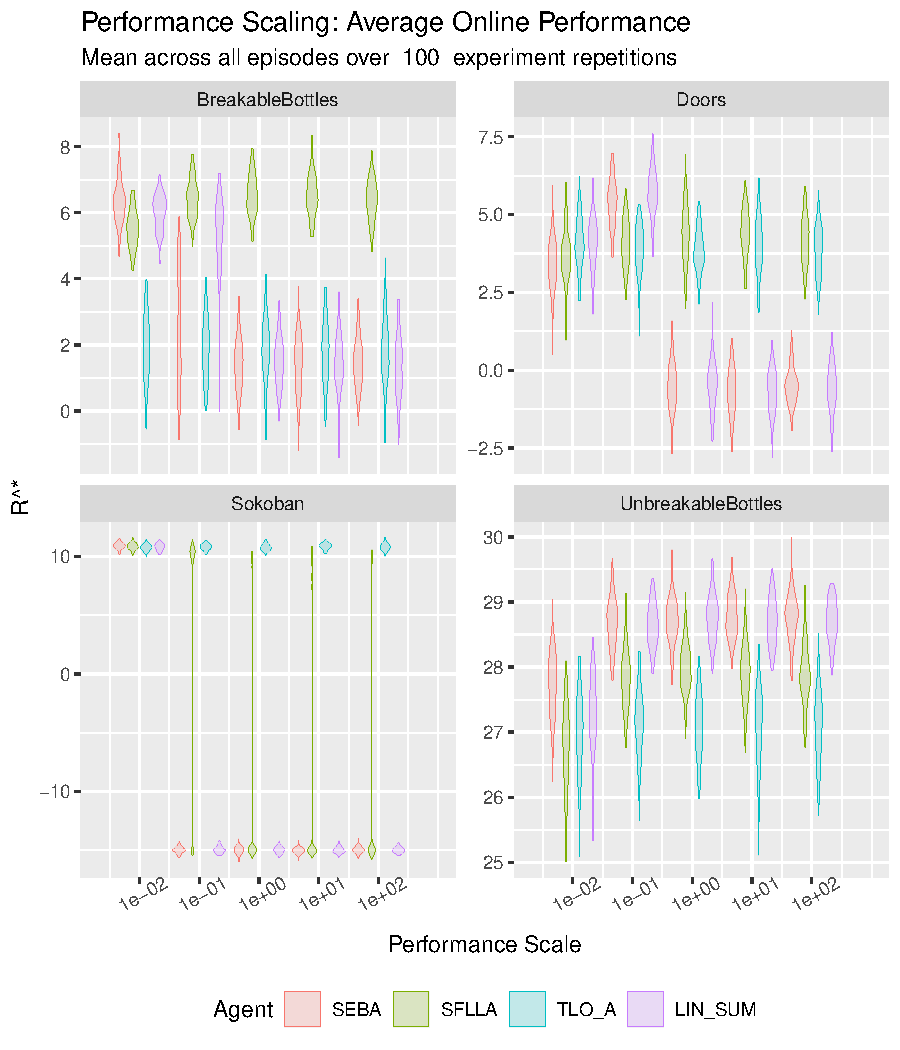
\includegraphics[width=\columnwidth]{output/multirun_n100_eeba_rolfonline_4agents_Performance.pdf}
  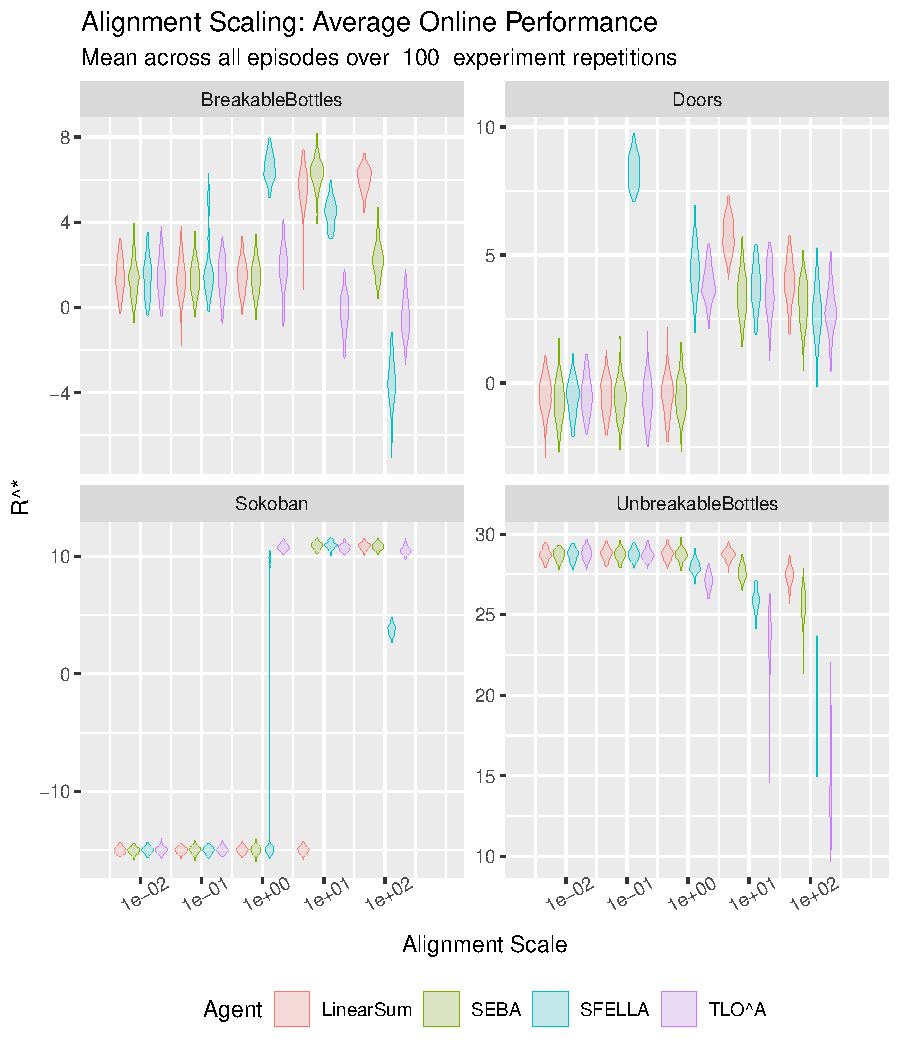
\includegraphics[width=\columnwidth]{output/multirun_n100_eeba_rolfonline_4agents_Alignment.pdf}
  \caption{Online performance averaged across learning episodes and experiment repetitions for different utility re-scales. (A): R* when scaling Performance across 5000 learning trials. Note SFELLA consistently performs similar or better to \tloA{}. (B): R* when scaling Alignment across 5000 learning trials. No algorithm is a clear best performer.%\footnote{what is the difference between top and bottom? both are online, but different objectives, right? include "top" "bottom" in caption}
  \rk{show Alignment and Performance rewards directly instead of R*, update y-axis description to say average reward (over epidodes and exp repetitions)}
  }
   \label{fig:online_performance}
   \Description{Online Performance and Alignment scaled performance}
 \end{figure}

While there was no clear best performer, SFELLA had the best online performance during training across a wider range of environments and environment variants than any other agent, including \tloA{}. Table~\ref{tab:mean_r_star_performance} describes relative $\text{R}^*$ scores for each function, compared to the $\text{TLO}^\text{A}$ function, at different scales.  Within the BreakableBottles environment, \tloA{} performed worse than all other agents at all scales, and SFELLA performed within 10\% of the best within five of nine scales. In the UnbreakableBottles Environment, performance between all agents except ELA was not significantly different. Agents in the Sokoban environment were generally very sensitive to scaling, though \tloA{} performed better in this environment overall. 



SFELLA tended to perform at best level when re-scaling the Primary objective (Figure~\ref{fig:online_performance}a), but less well when Alignment utility was re-scaled. (Figure~\ref{fig:online_performance}b).

